\documentclass{article}
\usepackage[T1]{fontenc}
\usepackage{lmodern}
\usepackage{graphicx}
\usepackage{amsmath,amssymb}
\usepackage[a4paper,margin=2cm]{geometry}
\usepackage[absolute,overlay]{textpos}
\setlength{\TPHorizModule}{1mm}
\setlength{\TPVertModule}{1mm}
\usepackage[indonesian]{babel}
\usepackage{hyperref}
\setlength{\emergencystretch}{2em}
% unit: Halaman 30

\begin{document}

% === Halaman 30 (python/native) ===

Istilah keilmuan 

serumpun terasa 

memberikan distorsi 

persepsi pada maksud 

sebenarnya. Persepsi 

yang segera terbentuk 

dengan istilah tesrebut 

adalah pertumbuhan dari 

akar-akar ilmu 

membentuk suatu 

rumpun, yang berarti 

bahwa nuansa historis 

organisasi/kelompok/unit 

yang mewadahinya. 






Embedded message 


Cover-image  


   Stego-image 

30

% deskripsi: gambar native xref 166
\noindent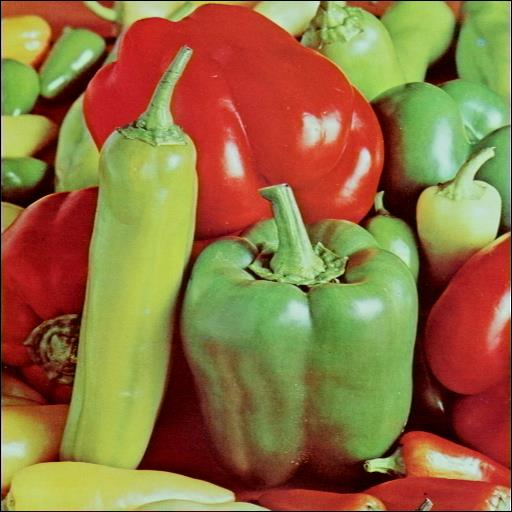
\includegraphics[width=0.85\textwidth]{../../images/python/page_030_img_01.jpeg}

% deskripsi: gambar native xref 167
\noindent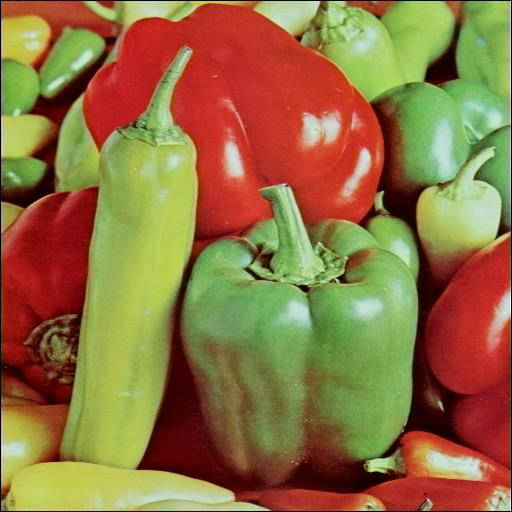
\includegraphics[width=0.85\textwidth]{../../images/python/page_030_img_02.jpeg}

\end{document}
